\documentclass[12pt, letterpaper]{article}
\usepackage[utf8]{inputenc}
\usepackage[margin = 1in]{geometry}
\usepackage[english]{babel}
\usepackage[superscript, biblabel]{cite}
\usepackage{verbatim}
\usepackage[section]{placeins}
\usepackage{booktabs}
\usepackage{float}

\usepackage[labelfont=bf]{caption}
\renewcommand{\abstractname}{\vspace{-\baselineskip}}
\usepackage{amsmath}
\usepackage{lipsum}
\bibliographystyle{naturemag}
\usepackage{graphicx}
\graphicspath{{../figures/}}
\setlength{\parindent}{0.5in}
\setlength{\parskip}{1em}
\usepackage{indentfirst}

\title{Mechanical Oscillators and Resonance \\
    \large Advanced Lab 2023}

\author{Seth White, John Meneghini}
\date{\today}

\begin{document}
    \maketitle

\centerline{\large Saint Vincent College}
\centerline{Department of Physics}

    \begin{abstract}
        The harmonic oscillator is a second order linear differential equation which describes many physical systems throughout physics and engineering. In this experiment we constructed a forced, damped harmonic oscillator and a coupled forced, damped harmonic oscillator and determined the resonance frequency of each system. The measured resonance frequencies were statistically different from the theoretical resonance frequency, which suggested the presence of damping in the systems.
    \end{abstract}
\newpage
	
    \section*{Introduction}
    Background

Radioactivity: 

Geiger M$\ddot$uller Tubes:
In this experiment, we will be using Geiger Muller tubes to measure radiation. Geiger Muller (GM) counters are the most widely used tool for radiation detection because of their accuracy and simple design.^1 A GM counter is able to detect alpha, beta, X-ray, and gamma radiation, giving it high versatility. Their internal construction is a cylindrical tube with a rod running down the center. The tube is filled with a gas, usually neon, argon, or helium, that will be ionized by radiation. A potential is applied between the tube and the inner rod, so that when radiation enters the chamber and ionizes the gas, there is a current flow between the tube and the rod. This current flow is detected by further circuitry and marked as a radiation detection event. In addition to the GM counter, we will be using a ST360 Radiation Counter to count and track radiation detections.


Radiation Shielding:

Goal
Find the dead time of the detector and the shielding coefficient

Overview
Operating Voltage, Background, Dead time, Radiation Shielding


Expected Relationship between shielding thickness and radiation attenuation
Functional Relationship:
Describe parameters you define in terms of their physical effects
Determine units for each parameter
Research that establishes its validity

1: Centric Geiger Muller Tubes 


    \section*{Methods}
    
\par \indent To run the experiment, we first had to determine the operating voltage for high sensitivity for the Geiger-$M\ddot{u}ller$ tube. This was done by sweeping the operating voltage from 0V - 1200V in 20V increments for 30 seconds. This data was then plotted to determine a range in which the operating voltage would be sensitive enough without causing dialectric breakdown and damaging the equipment. As seen in figure [], the operating voltage for high sensitivity is within the 800V-1100V range. Thus, 900V was chosen as it was within this range at a convenient point and agreed with the value provided by the manufacturer.

\par Once the operating voltage was determined, the background radiation count was measured to account for noise in the count rate. This was done by running the Geiger-$M\ddot{u}ller$ counter for 1000 runs at 1s intervals with no radioactive samples. This background count rate was then subtracted from each data set for count rate measured to minimize noise and gain more accurate results.

\par Another method in reducing the uncertainty for our experiment was calculating the dead time for the Geiger-$M\ddot{u}ller$ tube. Dead time is the period of time in which the positive ions take to reach the cathode and the tube becomes insensitive to radiation. Because count rates for radioactive samples are essentially random, we can attempt to correct this random statistical process to determine a true count rate of a substance.  Since the decay of radioactive nuclei can be described by a Poisson distribution, we relate the true count rate as
\begin{equation}
r = Re^{-RT},
\label{eq:ActualCountRate}
\end{equation}
where $r$ is the measured rate, $R$ is the true count rate, and $T$ is the dead time. If we take an approximation of this true count rate with a second-order Taylor Series approximation we see that
\begin{equation}
r \approx R(1-RT).
\label{eq:ApproxCountRate}
\end{equation}
Rearranging this for true count rate, we have that
\begin{equation}
R \approx \frac{r}{1-rT}
\label{eq:TrueCountRate}
\end{equation}

\par By accounting for the dead time in our experiment, we can calculate the true count rate of a radioactive sample. This is done by implementing the two-source method. When combining two sources, we measure the combined activity, $r_3$, as 
\begin{equation}
r_1 + r_2 = r_3 + b,
\label{eq:combinedcountrate}
\end{equation}
where $r_1$ and $r_2$ are the individual counts and $b$ is the background count. If each count rates are corrected for dead time, the previous equation becomes
\begin{equation}
\frac{r_1}{1-r_1 T} + \frac{r_2}{1-r_2 T} = \frac{r_3}{1-r_3 T} + b.
\label{eq:cominedwithdeadtime}
\end{equation}
The background count is not corrected because it is already negligible as is. This means we can transform the equation for dead time into a quadratic by
\begin{equation}
r_1 r_2 r_3 T^2 - 2r_1 r_2 T + r_1 + r_2 - r_3 = 0.
\label{eq:quaddeadtime}
\end{equation}
Because $T$ is roughly on the order of microseconds, we can also negate the $T^2$ term and reduces the equation to the final dead time calculation of 
\begin{equation}
T = \frac{r_1 + r_2 - r_3}{2r_1 r_2}.
\label{eq:deadtime}
\end{equation}
To determine dead time through this two-source method, we used one Co-60 source and one Cs-137 source and measured both individual count rates. Then both sources were measured together, roughly stacked on top of each other since we did not have half-sources, for the total count rate. Then the dead time was calculated by the above equation.

%Taken from Sam
\par Using the true count rate calculated by the measured dead time, we can use this value to understand how gamma ray radiation interacts with different materials. We expect the radiation attenuation through a material to follow an exponential decay as a function of thickness. The intensity $I$ after passing through a lead shield of thickness $X$ is given by the equation
\begin{equation}
I = I_0e^{-\mu X},
\end{equation}
where $I_0$ is the initial intensity and $\mu$ is the attenuation coefficient. To solve for $\mu$, we set the final intensity equal to half the initial intensity, which will occur after a thickness $X_{1/2}$, the half thickness:
\begin{equation}
1/2 I = I_0e^{-\mu X_{1/2}}.
\end{equation}
Solving Equation (2) for $\mu$ gives
\begin{equation}
\mu = ln(2)/{X_{1/2}}.
\end{equation}
 Varying different thickness of lead shielding and measuring the resulting count rate, we determine the relationship between attenuation and material thickness.



	\newpage
    \section*{Data and Results}
    \begin{figure}[H]
	\centering
	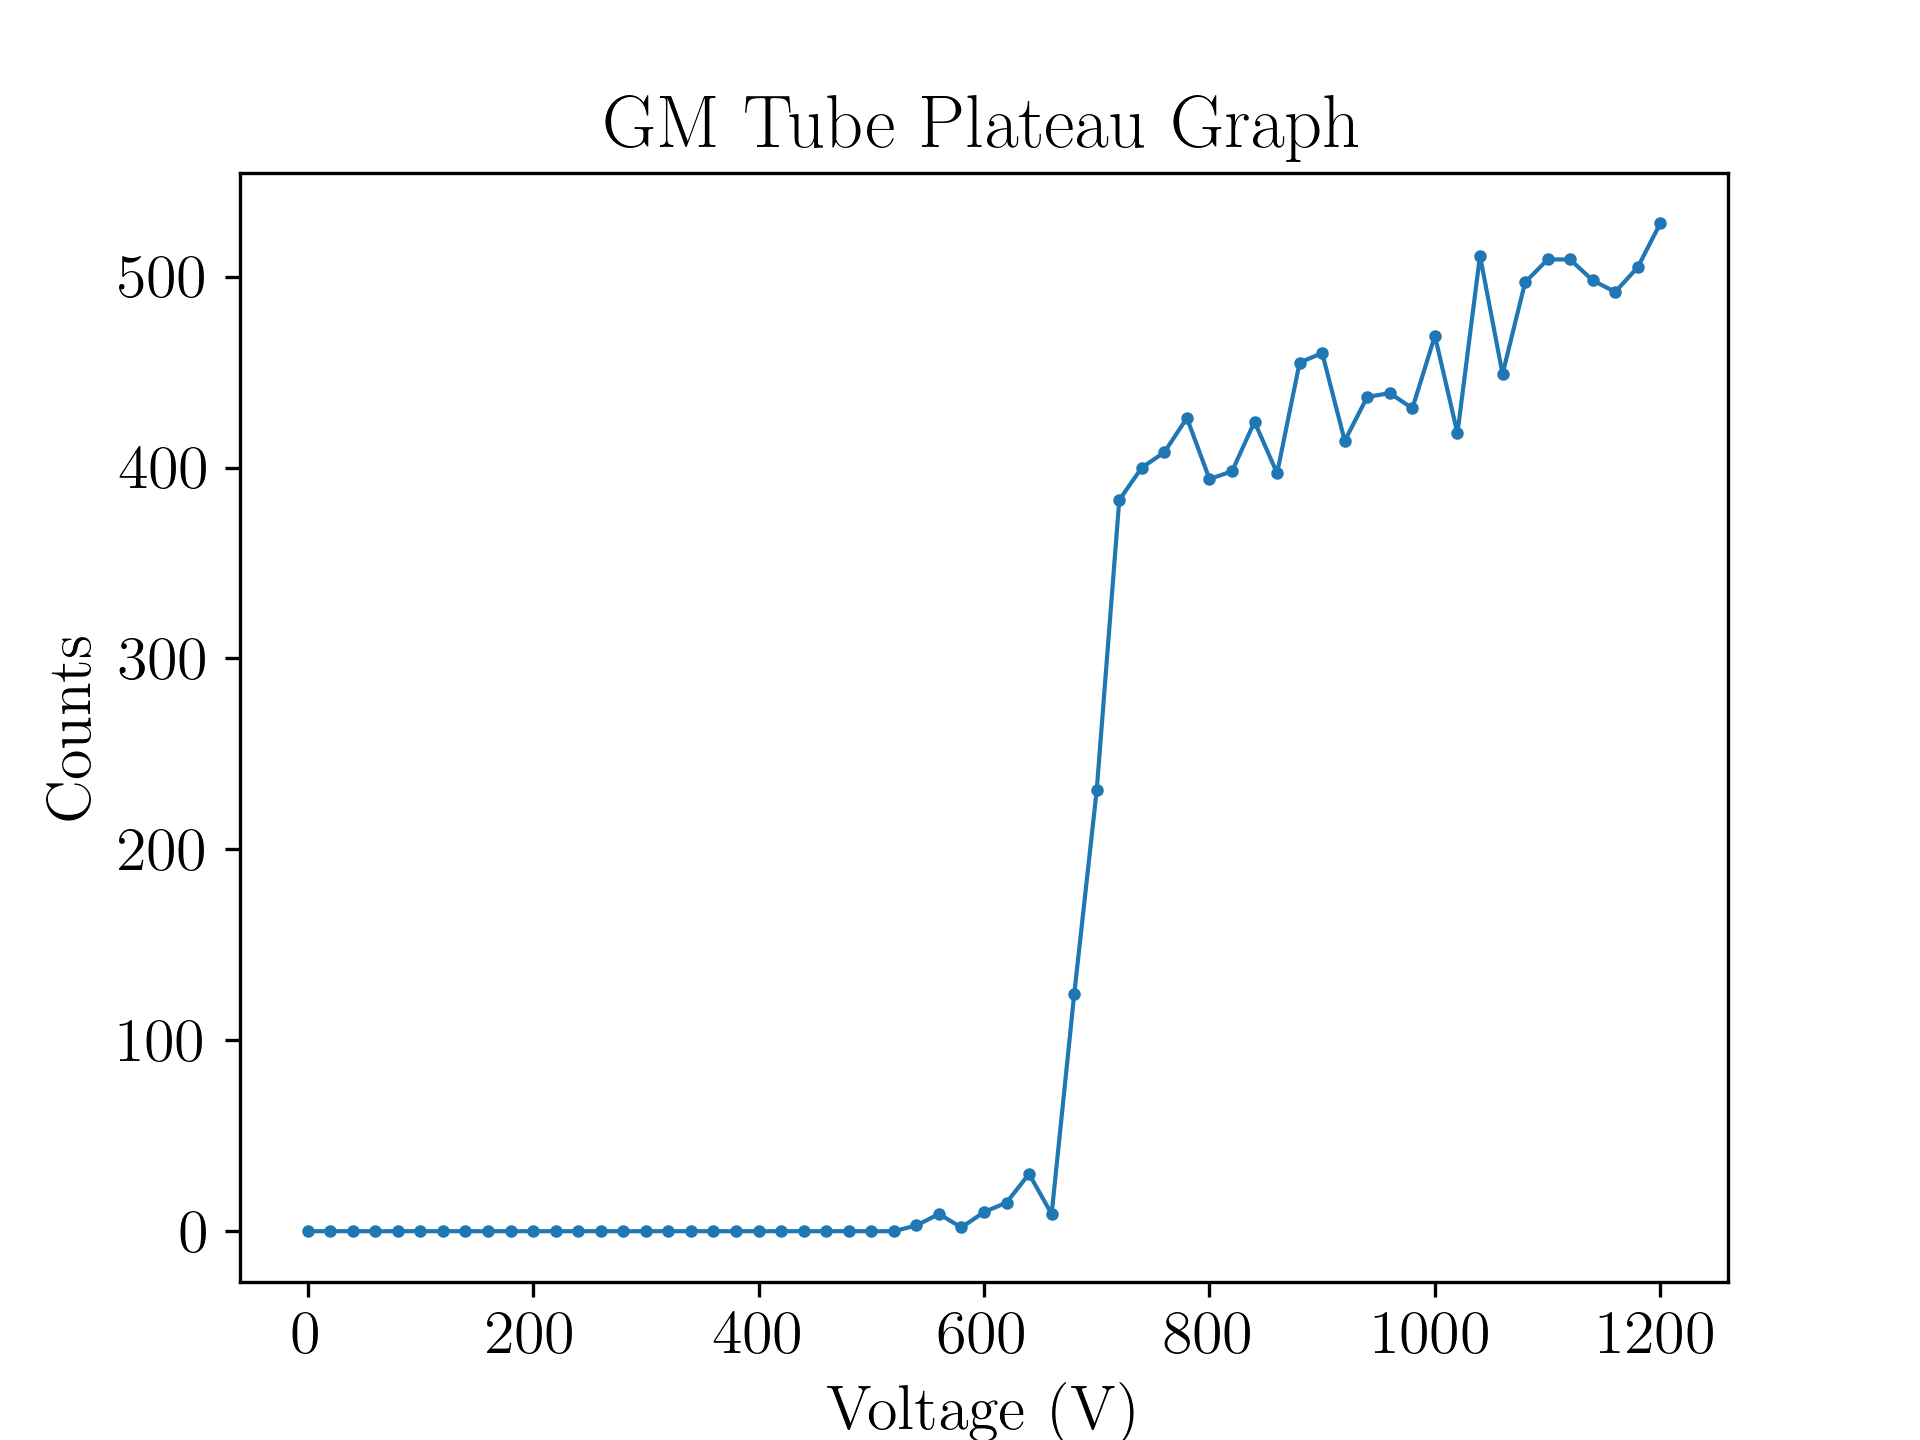
\includegraphics[scale=1]{PlateauGraph.png}
	\caption{Counts vs. Voltage (V) for the plateau curve experiment, where the operating voltage of the Geiger-Muller tube was increased by 20 V from 0 V to 1200 V.}
\end{figure}

\begin{figure}[H]
	\centering
	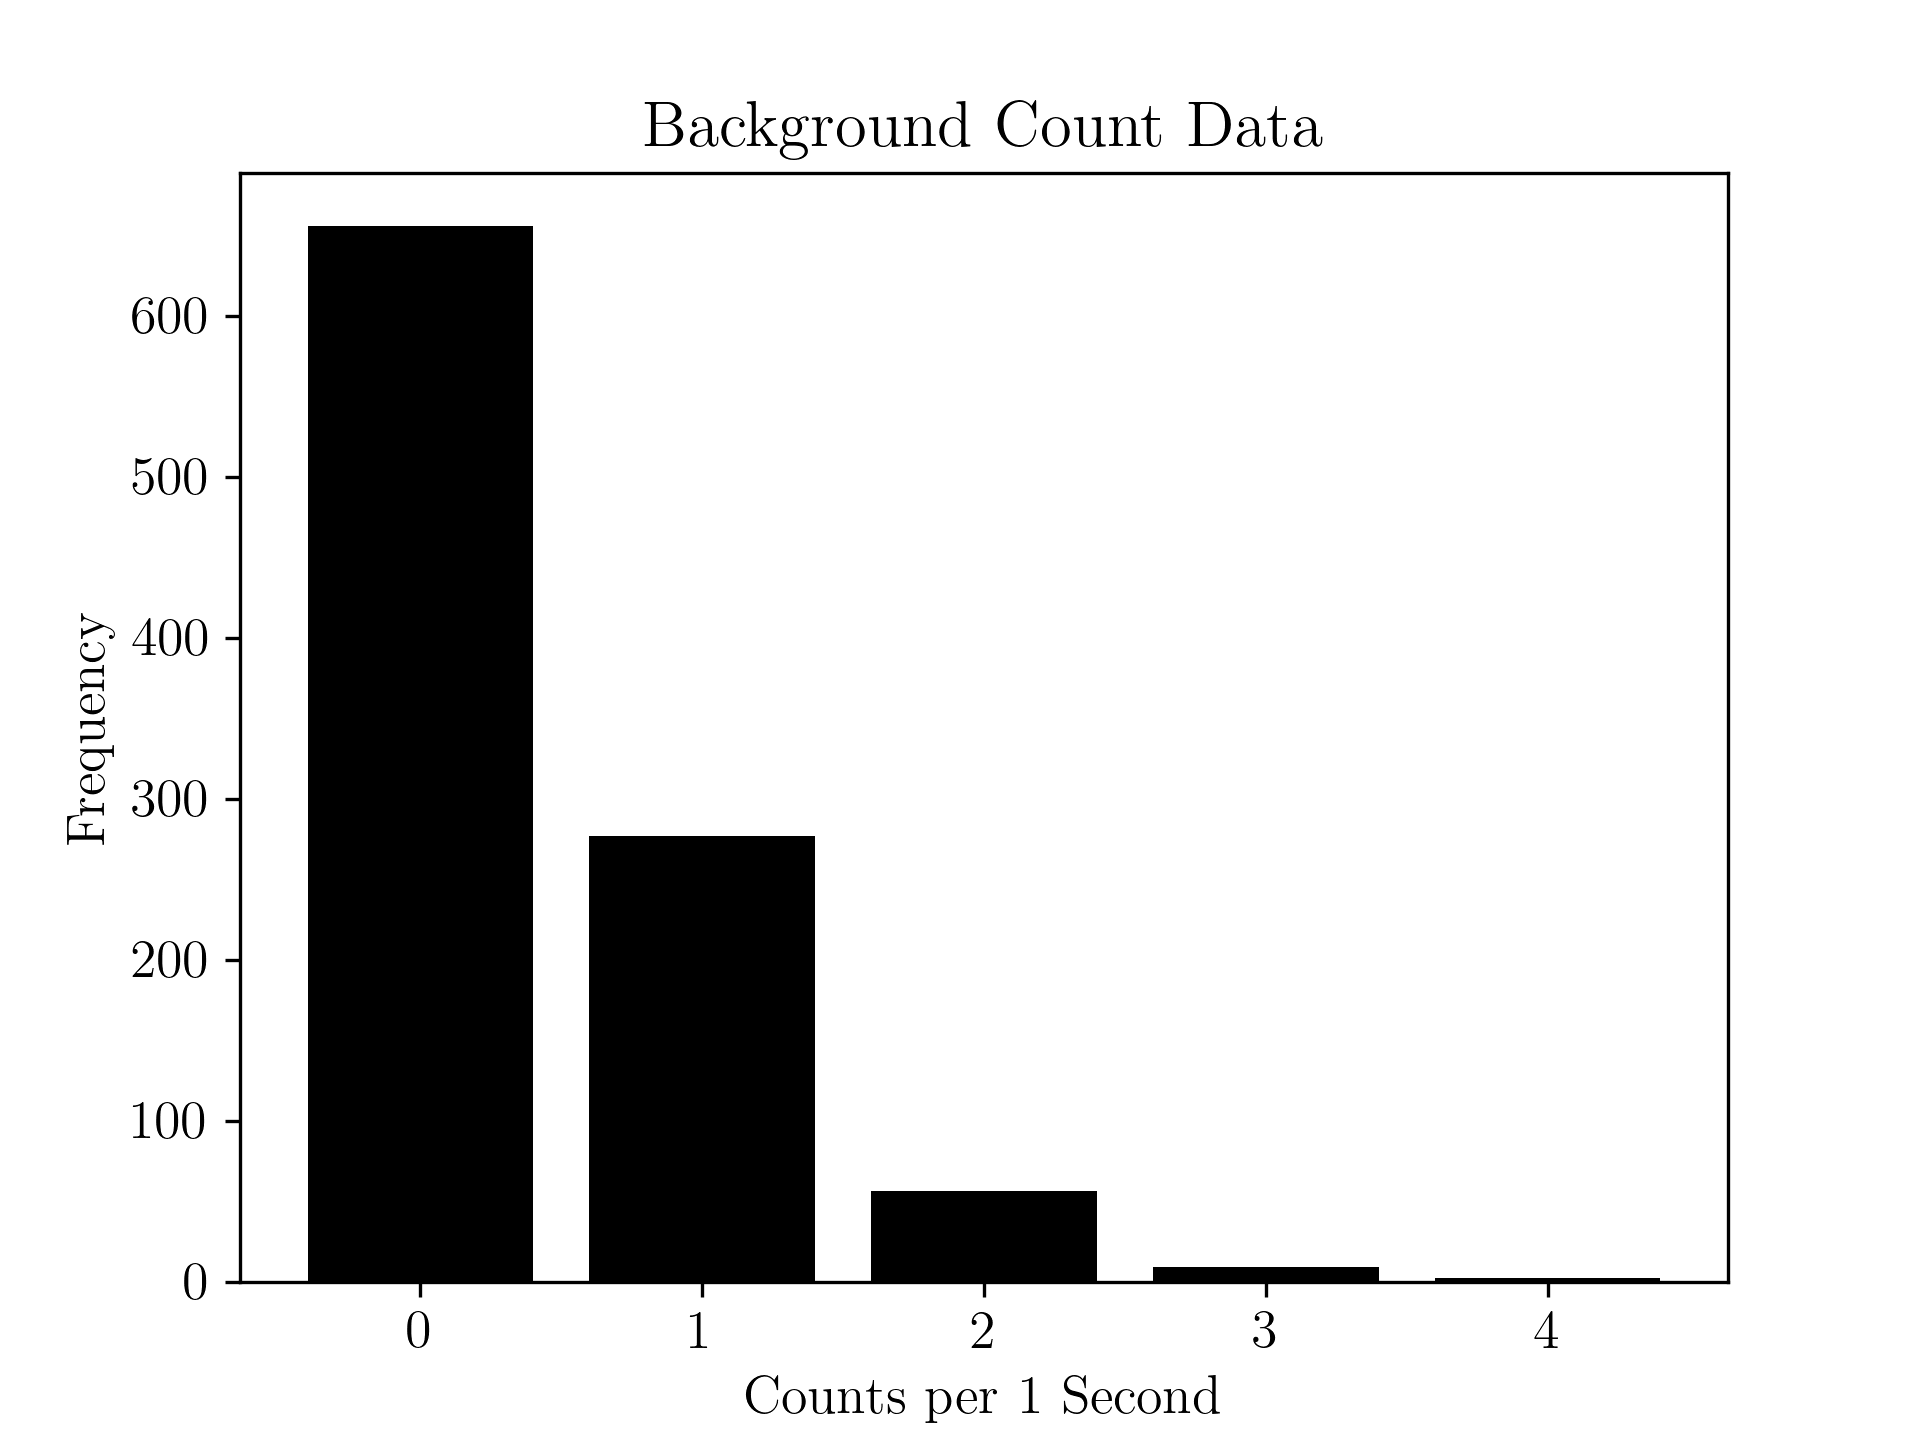
\includegraphics[scale=1]{BackgroundCountHist1sec.png}
	\caption{Count distributions over intervals of 1 second for the background measurement.}
\end{figure}

\begin{figure}[H]
	\centering
	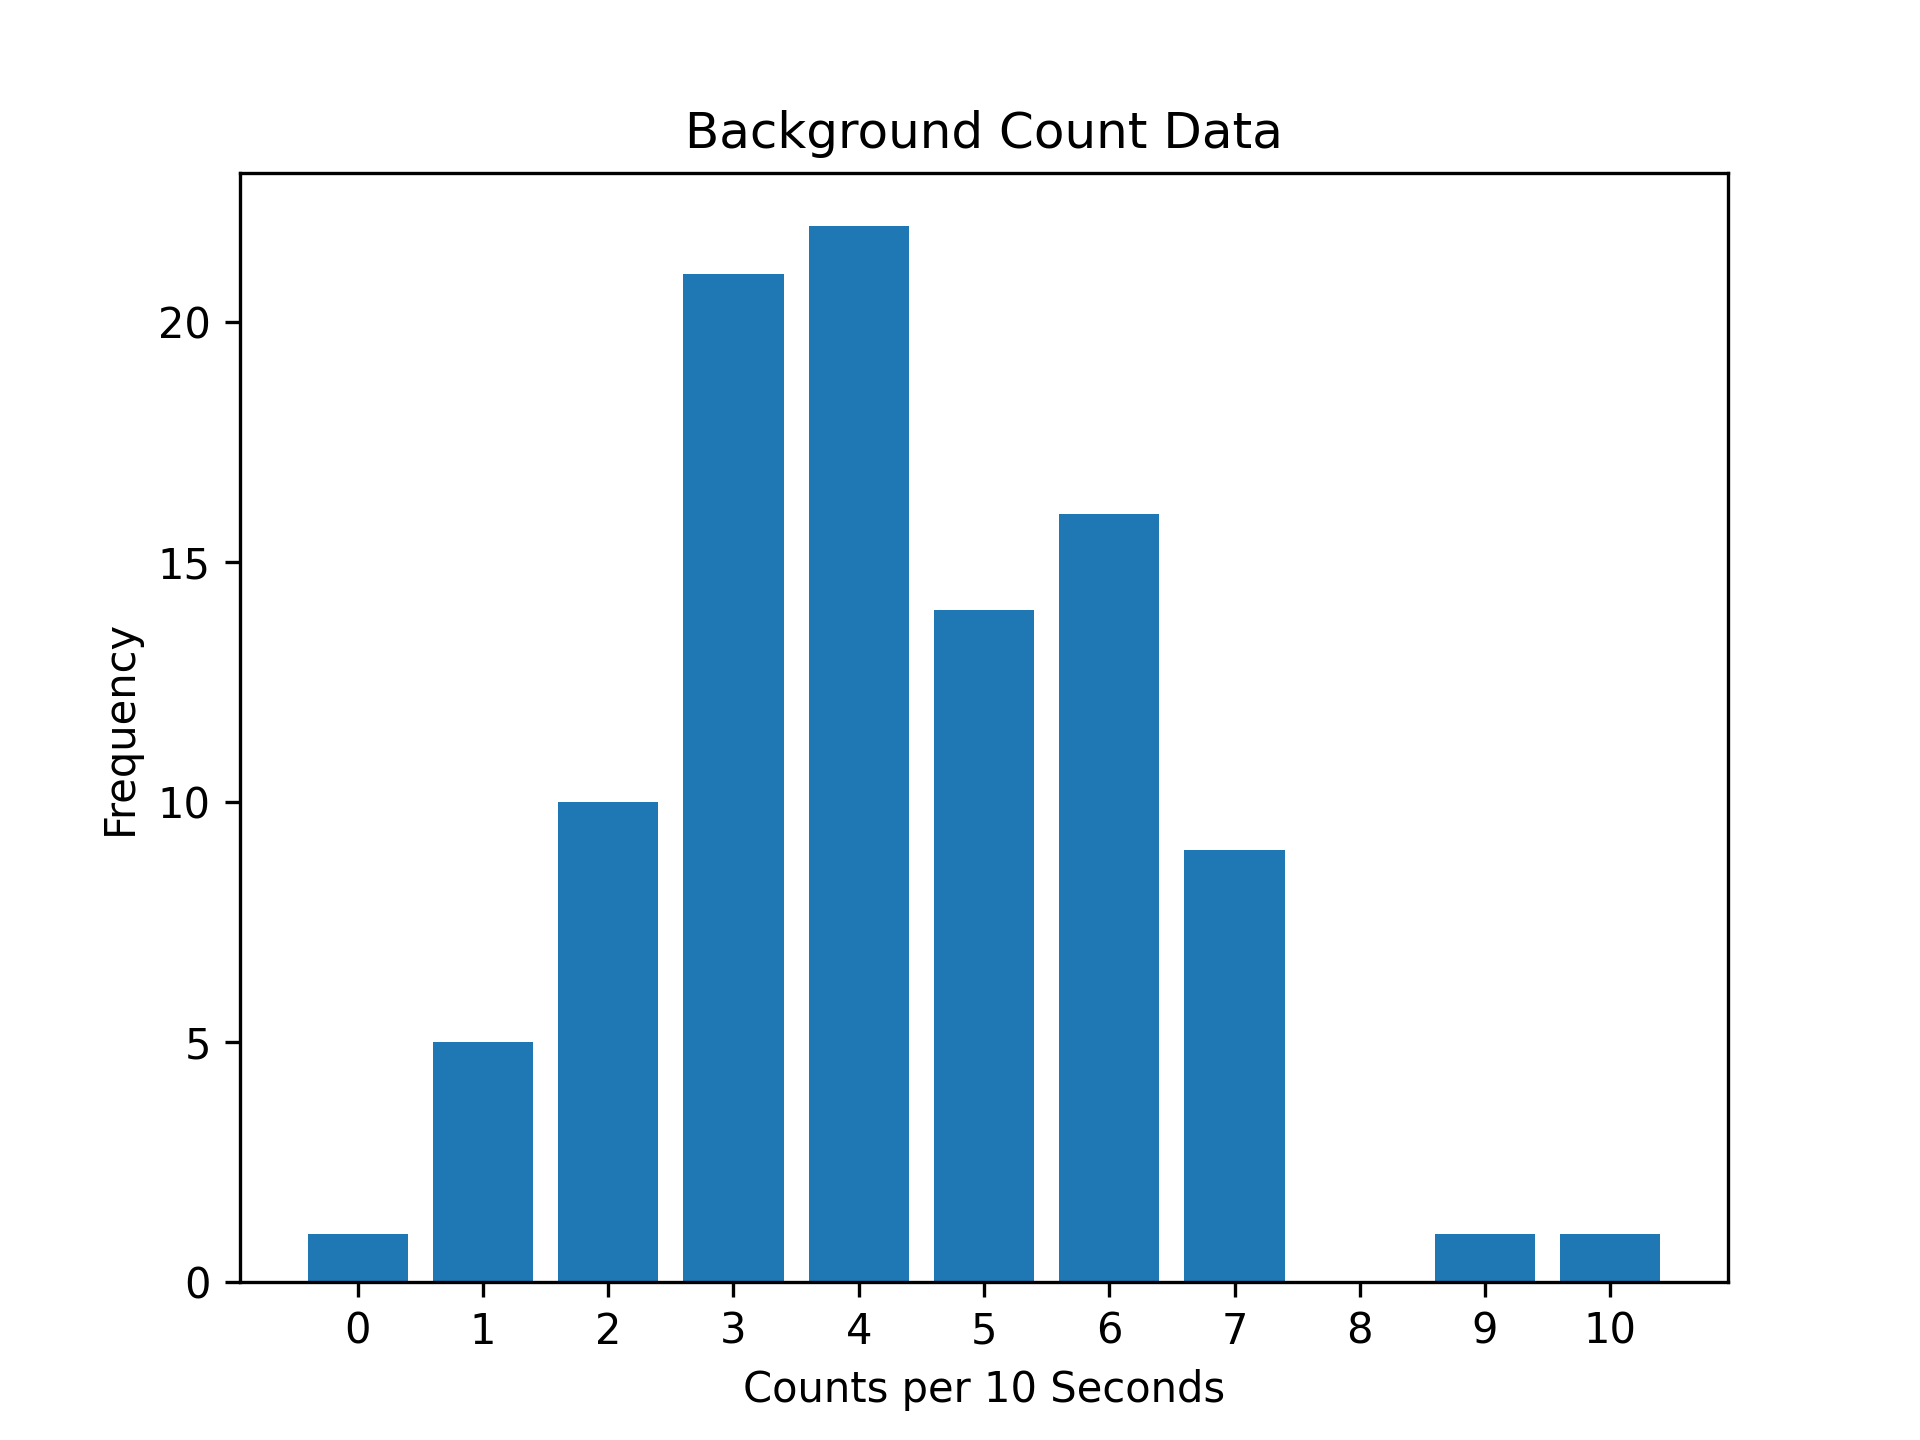
\includegraphics[scale=1]{BackgroundCountHist10sec.png}
	\caption{Count distributions over intervals of 10 seconds for the background measurement.}
\end{figure}

\begin{figure}[H]
	\centering
	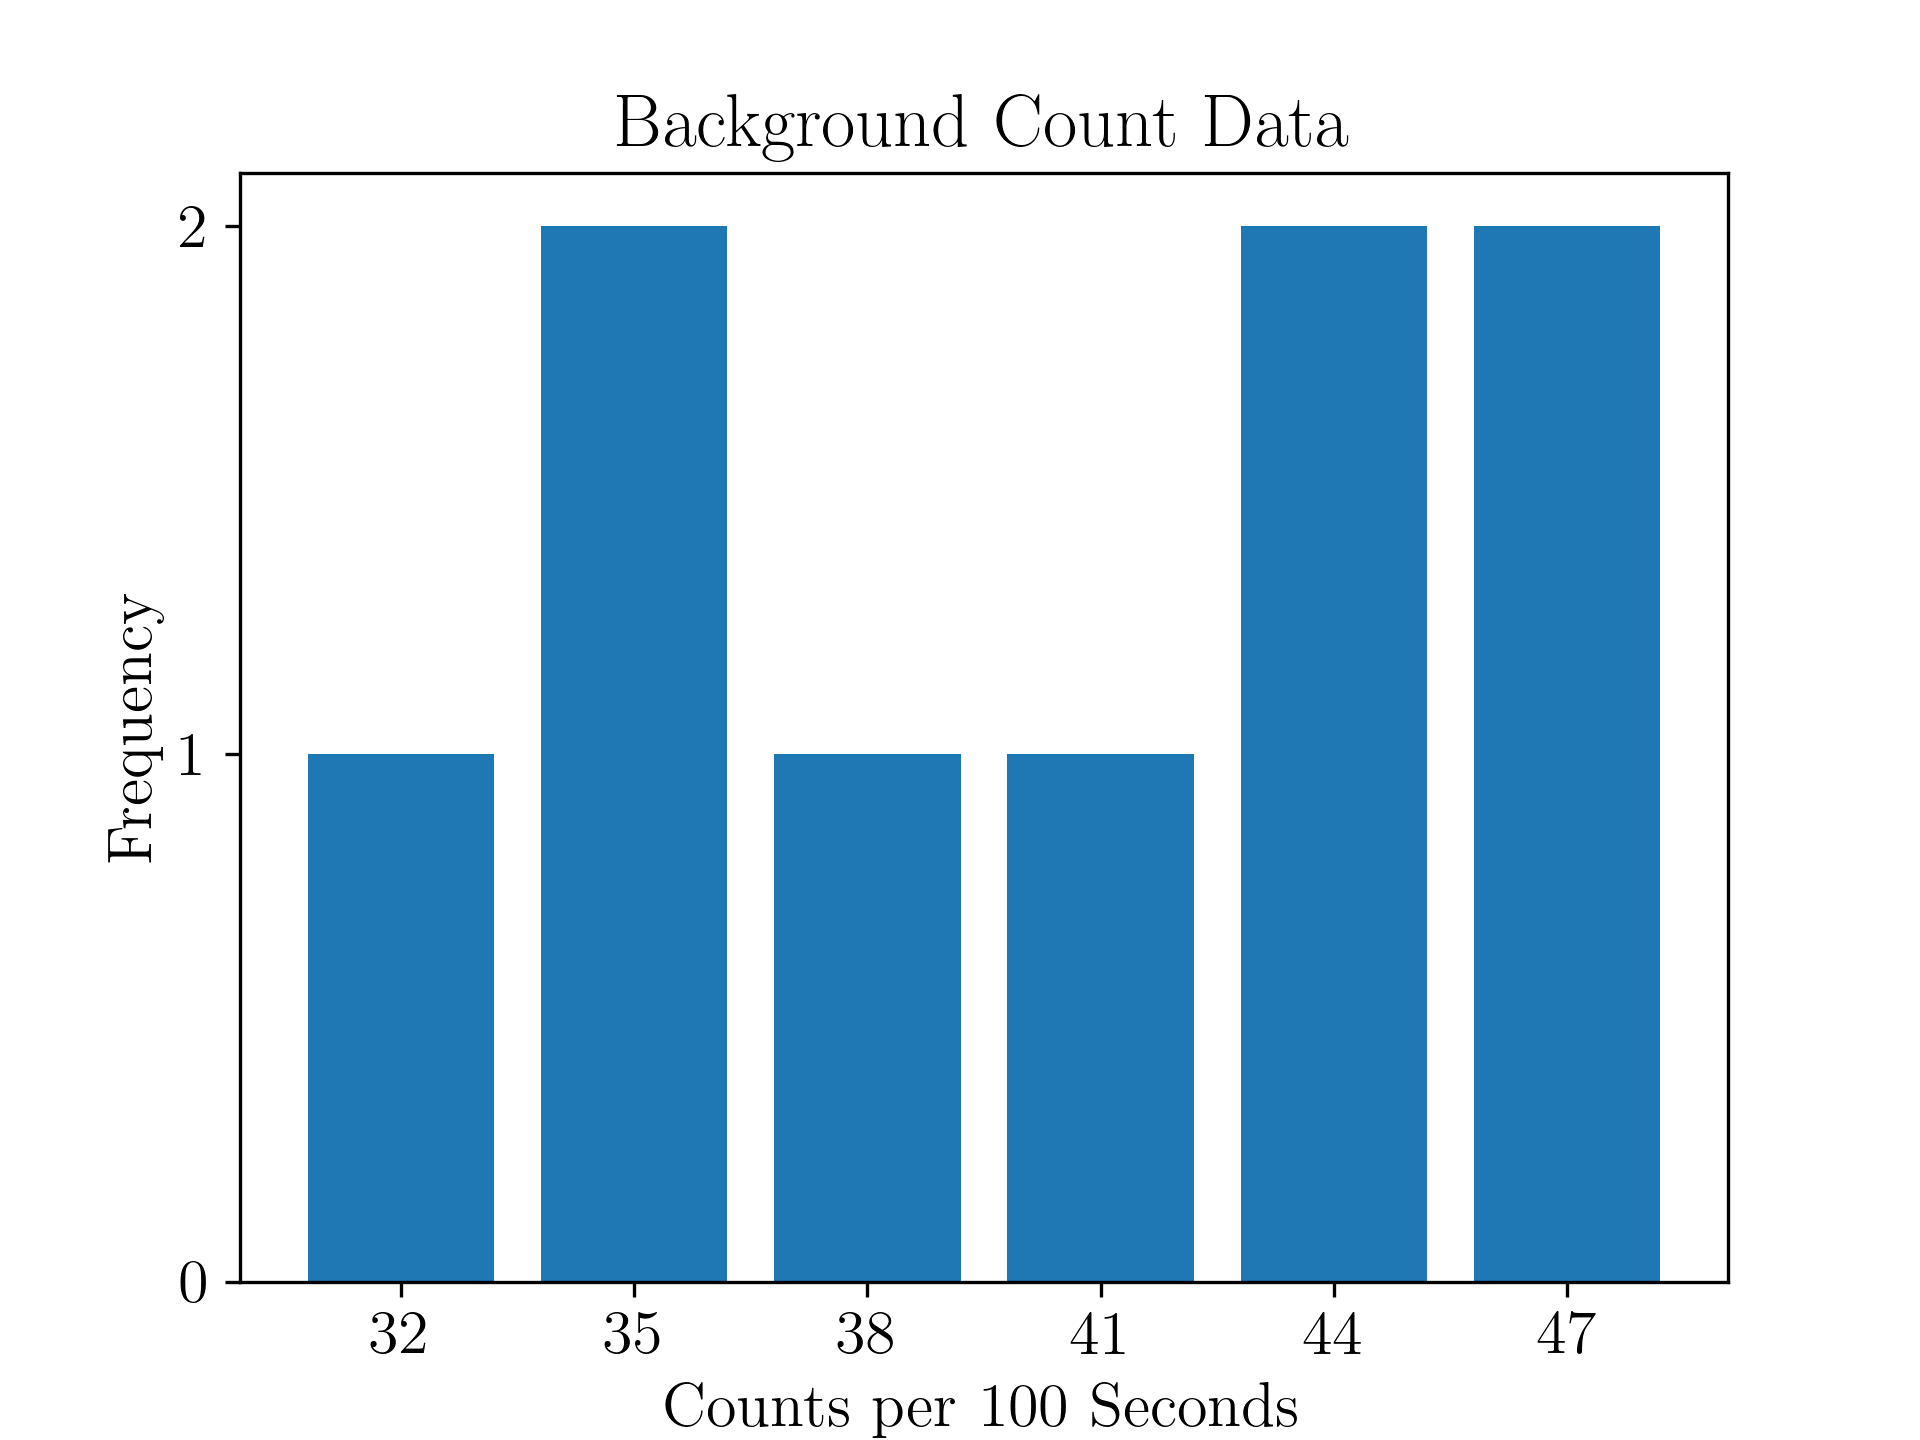
\includegraphics[scale=1]{BackgroundCountHist100sec.png}
	\caption{Count distributions over intervals of 100 seconds for the background measurement.}
\end{figure}

\begin{table}[H]
    \centering
    \captionof{table}{Count and count rate data for the $^{60}$Co shielding experiment} \label{tab:at} 
    \begin{tabular}{ccccc}
\toprule
 d (mm) &  Total Counts &  Total Counts Std. &  Count Rate (Bq) &  Count Rate Std. (Bq) \\
\midrule
 0.0000 &       29669 &         200 &        19.8 &              0.1 \\
 1.6256 &       22194 &         100 &        14.8 &              0.1 \\
 3.1750 &       20293 &         100 &        13.5 &              0.1 \\
 6.3500 &       17420 &         100 &        11.6 &              0.09 \\
\bottomrule
\end{tabular}

\end{table}

\begin{figure}[H]
	\centering
	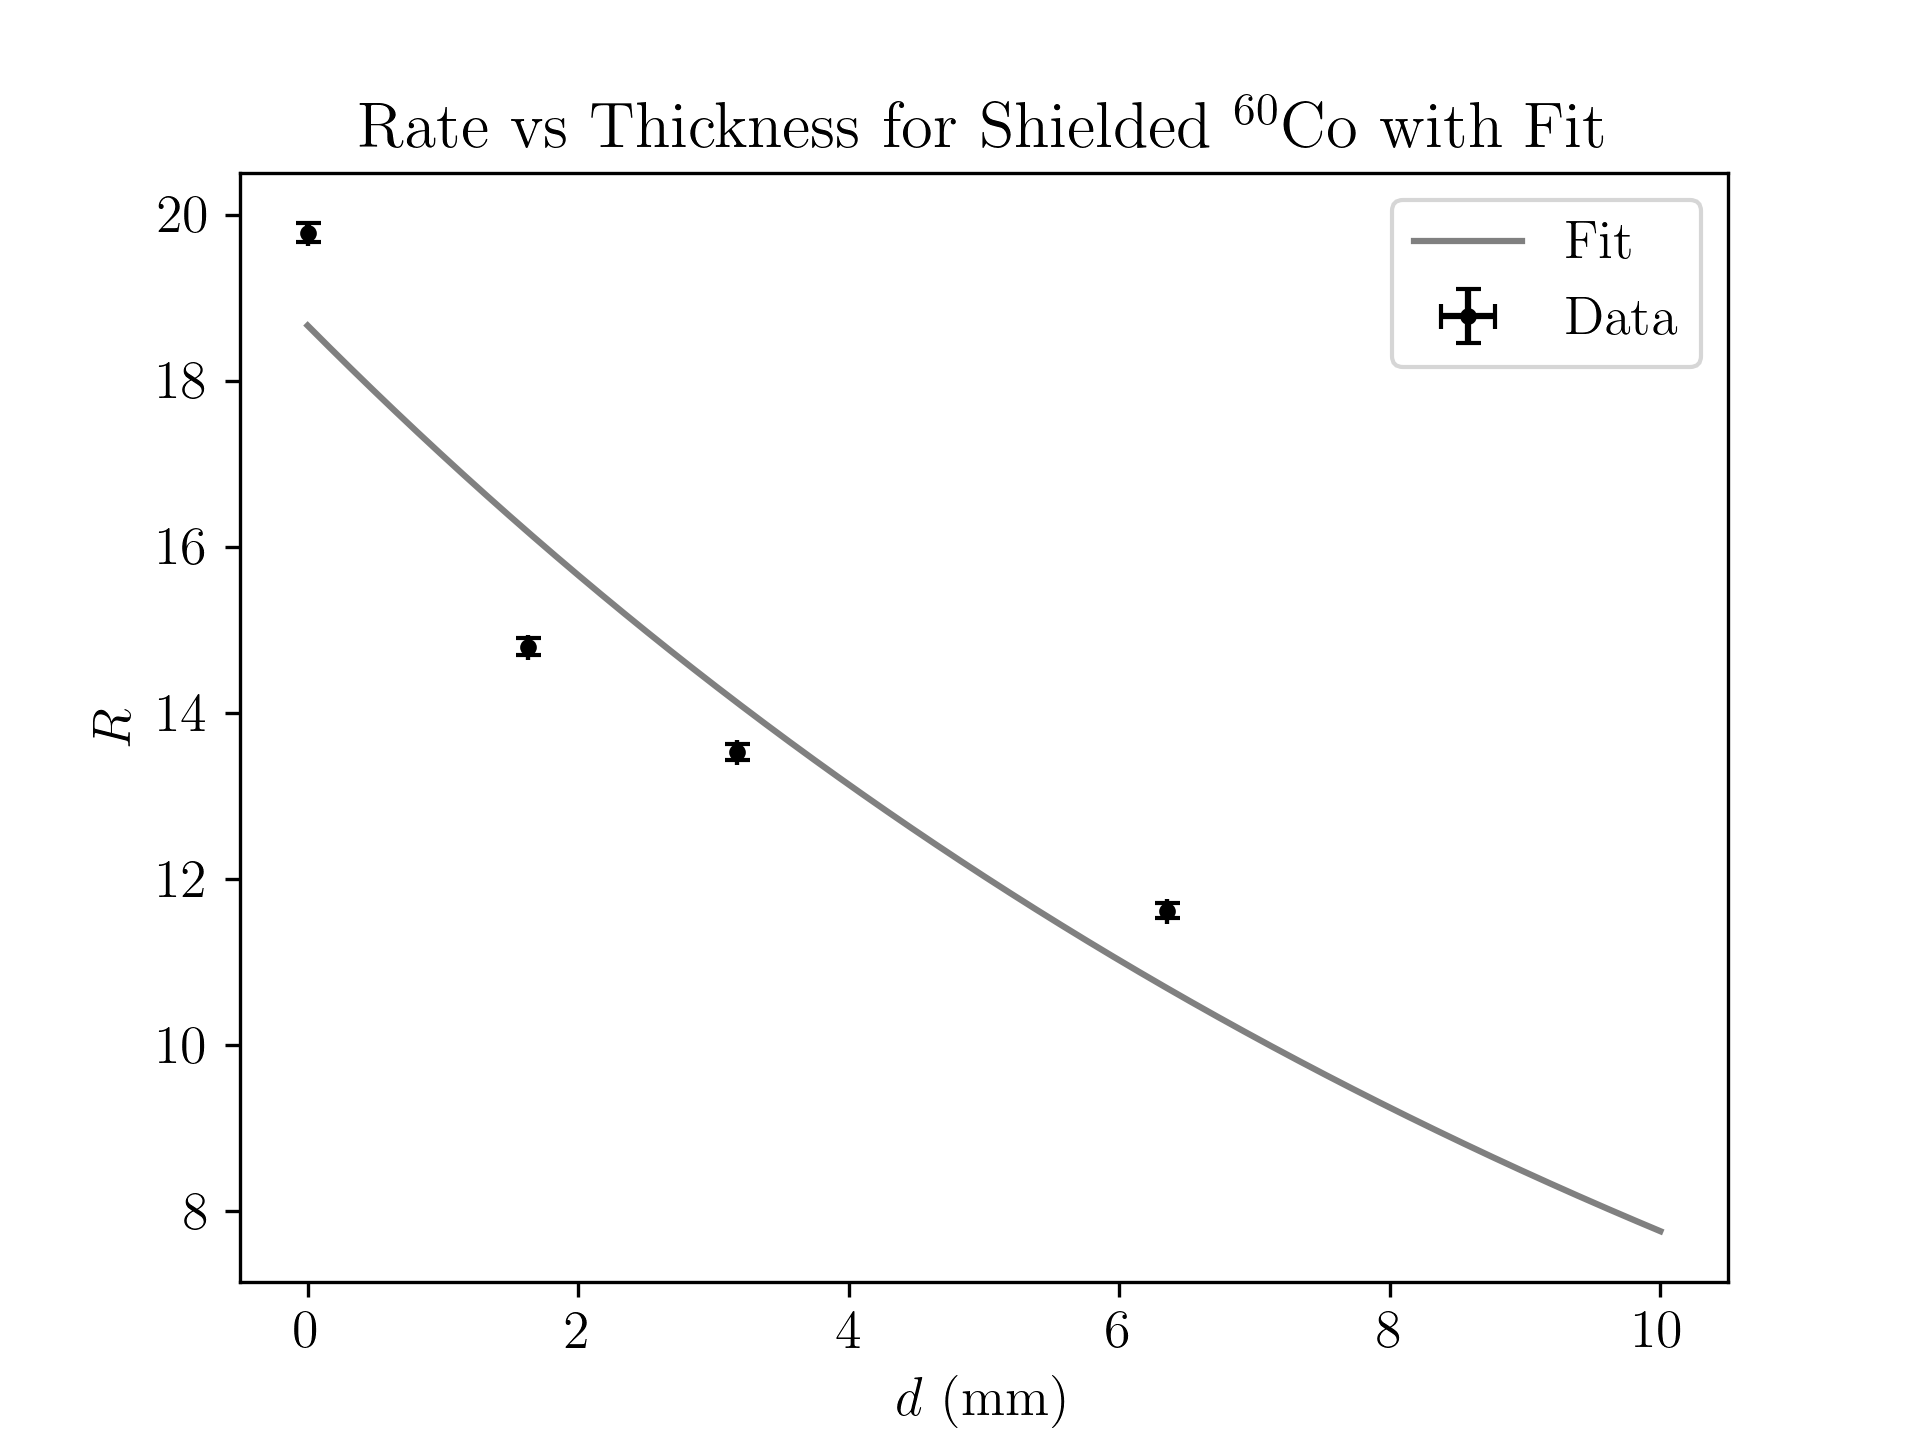
\includegraphics[scale=1]{co60_rate_vs_thickness_fit.png}
	\caption{Rate (Bq) vs shielding thickness (mm) for the shielding experiment using $^{60}$Co. Fitted using the equation $R = R_0 e^{-d/d_0})$, resulting in $R_0 = 18.663 \pm 0.3$ Bq and $d_0 = 11.387 \pm 0.8$ mm.}
\end{figure}

\pagebreak





	\newpage
    \section*{Discussion}
    \par In all three experiments, the amplitude resonance frequencies measured were less than the theoretical values. This would suggest that a damping factor was still observed on the air track during the experiment. In all theoretical calculations, the increase of damping factor would reduce the natural frequency as can be seen in the derivation of the single cart resonance frequency in equation (\ref{eq:naturalfreq}).

\par This damping could possibly have been caused by some friction on the air track still present in the experiment. The experiment where we added the weight to the single air cart system showed the greatest deviation from theoretical value. For the track to account for this gain in mass, the air track would have to produce a stronger output of air; this was impossible due to the experiment being run on the highest setting for the pump throughout. Another possibility could be the presence of turbulence under the carts. Because the system is moving and changing the direction constantly, the air has difficulty escaping and may get trapped and cause small changes in the air cart as it oscillates on the track. 

\par Due to the possibility of damping in the system, the observed maximum amplitudes might not have been the theoretical maximum possible in the system. From this we could estimate the damping factor $\gamma$ by relating the difference of theoretical resonance frequency to the measured resonance frequency of the system. This would be slightly unreliable because of the possibility that the maximums arent truly being measured as suggested. Therefore multiple factors of uncertainty would render this estimate difficult.

\par Though the maximum amplitudes were not achieved, the coupled, damped harmonic oscillator still demonstrated both resonance frequencies. Another common reference of these resonance frequencies are the symmetric and the asymmetric resonance. This is due to the way the carts oscillate in reference to each other. The carts moved for one frequency back and forth together in the same direction (asymmetric), and then opposite direction for the other frequency (symmetric). This nomenclature makes sense with reference to a center axis between the two carts.

    \newpage
    \bibliography{main.bib}
\end{document}
